\documentclass[10pt]{article}
\usepackage{amsmath} 
\usepackage{graphicx}
\usepackage{enumerate}

\usepackage{geometry}
\geometry{legalpaper, margin=1in}

\usepackage{mdframed}

\graphicspath{{../figs/}}


\begin{document}

\title{Simulaciones del modelo de Ising en 2D}

\maketitle


Considere el modelo de Ising en la red cuadrada de $L \times L$ sitios (parámetro de red unitario) con interacciones entre primeros vecinos:

\begin{equation}
H = - J \sum_{\langle i,j\rangle} S_i S_j - B \sum_i S_i.
\end{equation}

Usando condiciones de contorno periódicas y tomando la energía en unidades de $k_B$ (esto es, tomando $k_B = 1$) implemente un programa para simular las propiedades termodinámicas del modelo usando el algoritmo de Metropolis. Mediante este programa realice los siguientes cálculos:


\pagebreak

\begin{enumerate}[a)]

\item A campo nulo calcule las curvas de magnetización ($\langle |m| \rangle_L$), susceptibilidad y calor específico en función de $T/J$, para tamaños $L = 16, 32, 64, 128, \text{ y } 200$. Para cada magnitud grafique simultaneamente las curvas correspondientes a los diferentes tamaños. En el caso de la magnetización y el calor específico grafique también la solución exacta para la red infinita. Calcule en las mismas simulaciones las cantidades $\langle m^2 \rangle_L$ y $\langle m^4 \rangle_L$. Recuerde que cerca de la temperatura crítica los tiempos de relajación al equilibrio aumentan. Realice algunos tests preliminares.

\begin{figure}[ht]
\centering
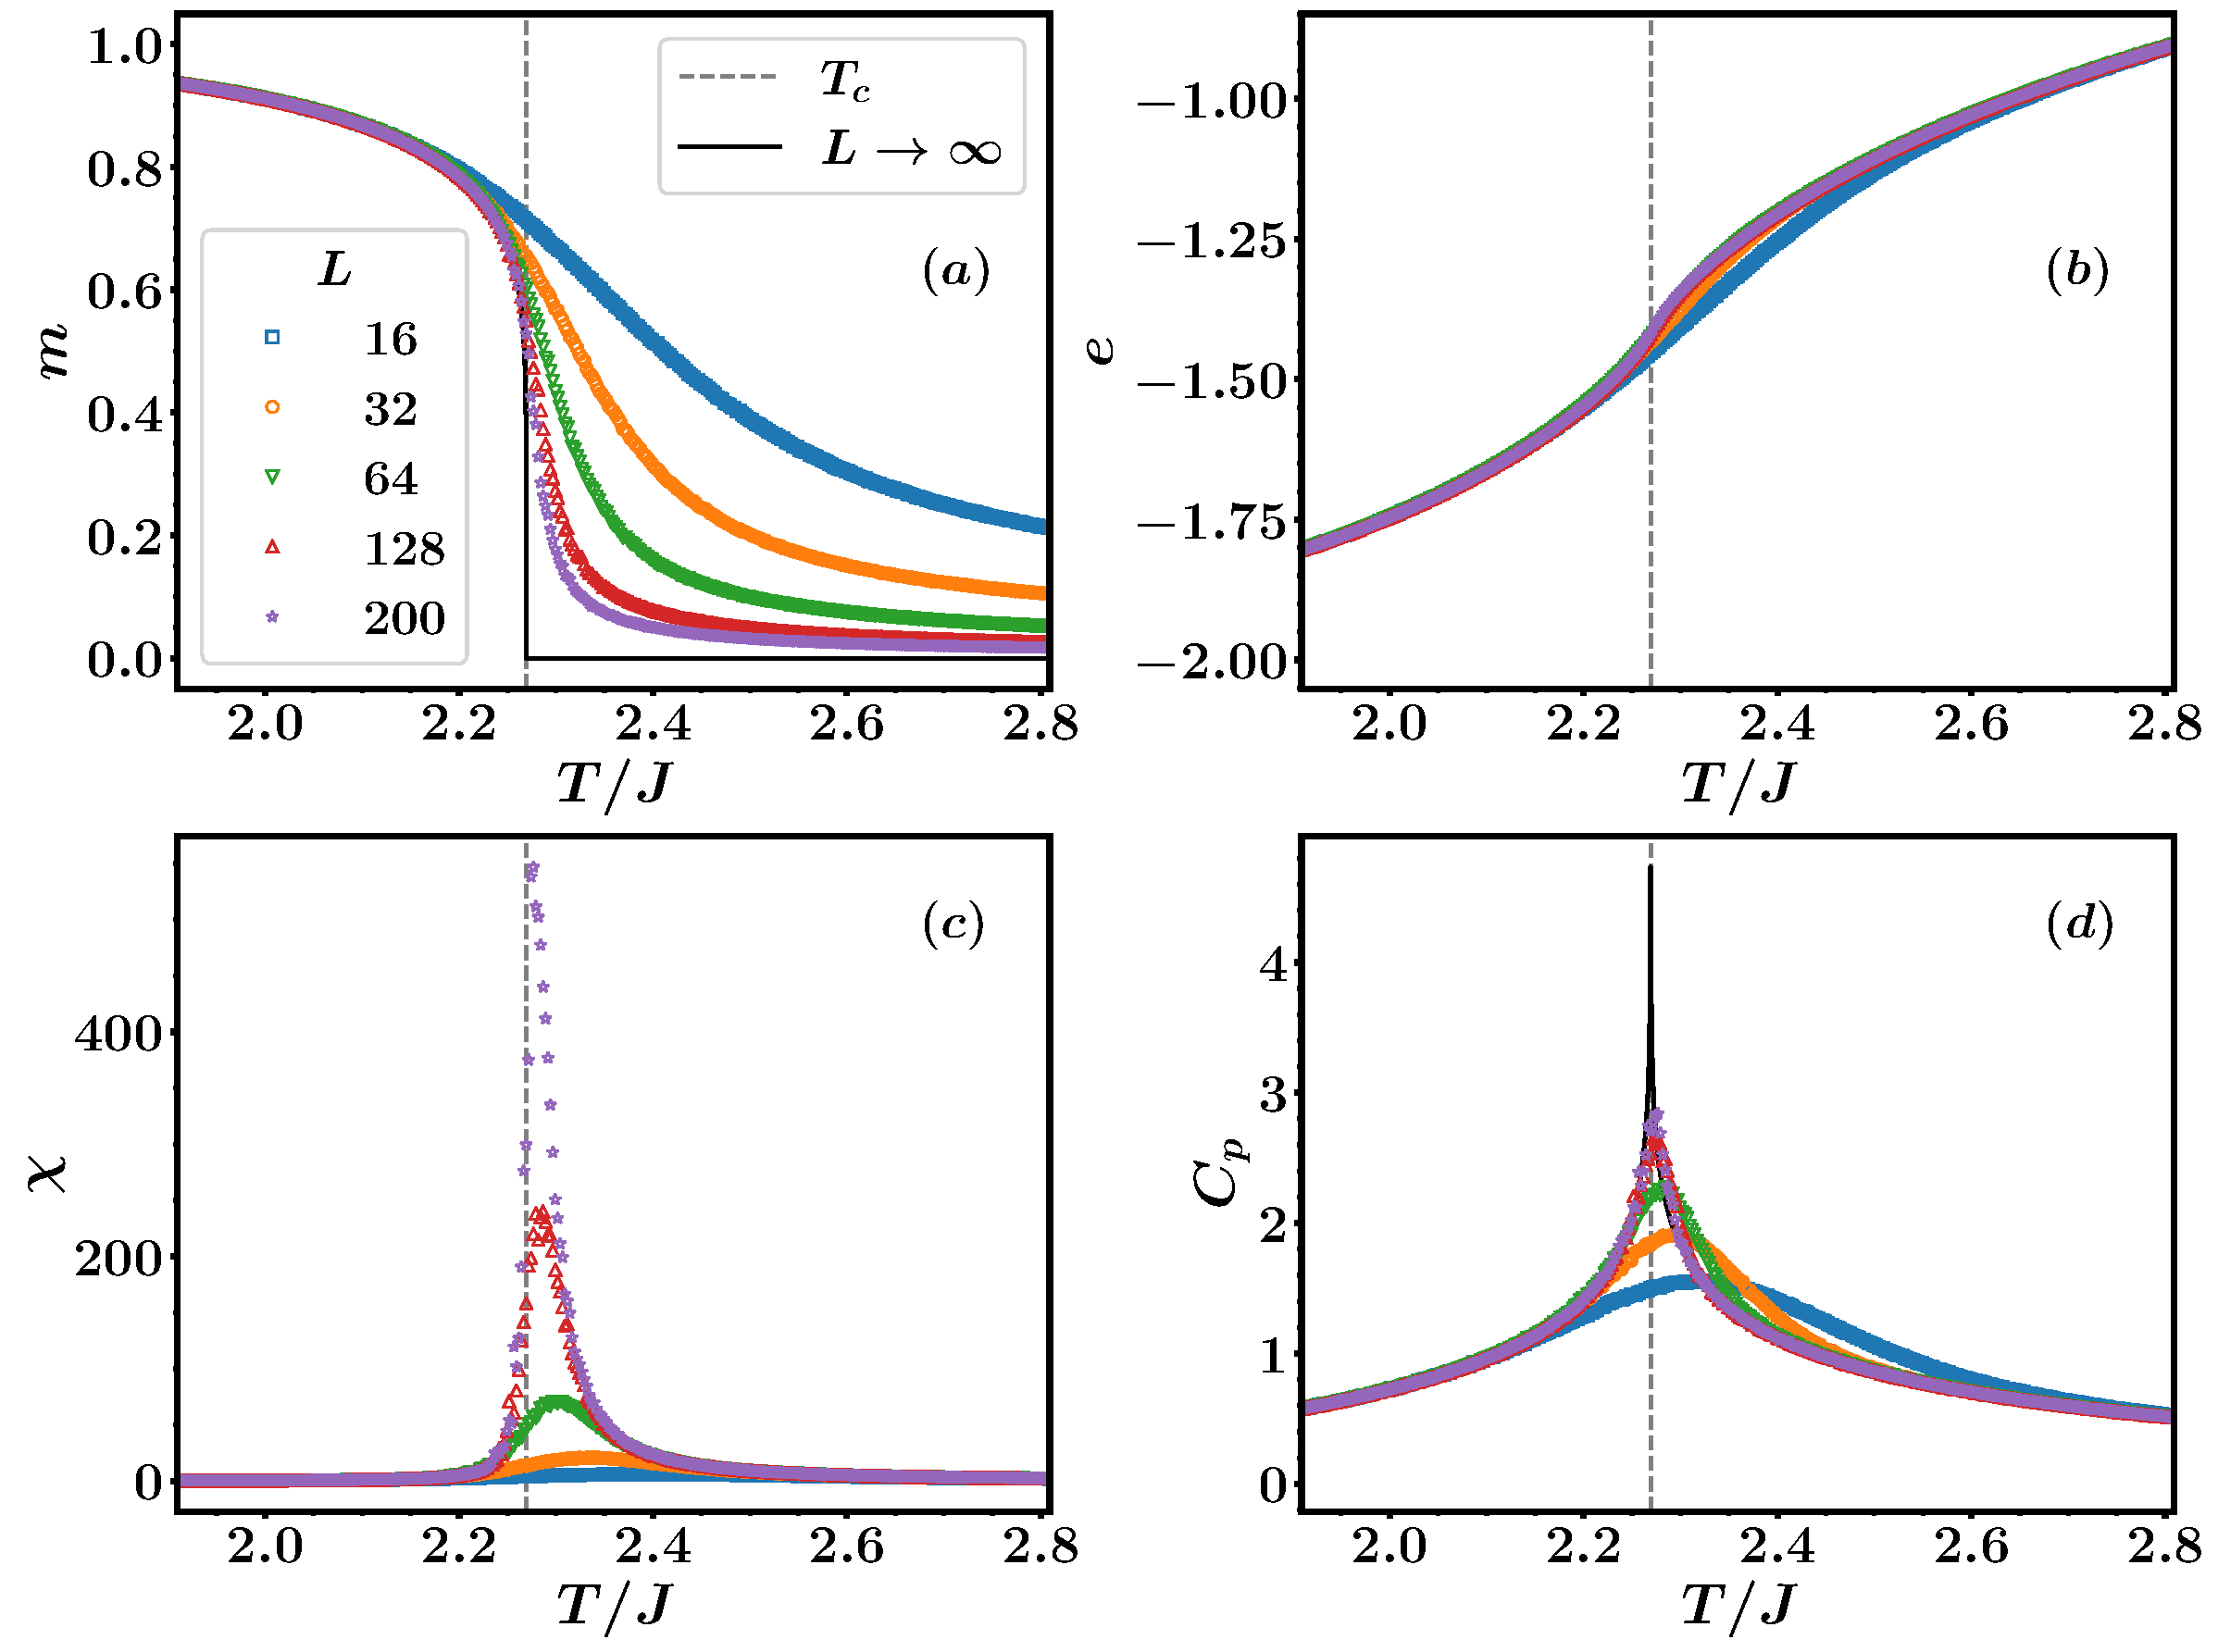
\includegraphics[scale=0.27]{Fig1.pdf}
\caption{Distintas magnitudes como función de la temperatura para distintos tamaños. (a) Magnetización, (b) Energía, (c) Susceptibilidad, (d) Calor específico. Podemos ver que, a medida que el tamaño del sistema aumenta, la transición se vuelve más abrupta, aproximandose a la solución teórica, correspondiente a tamaño infinito.}
\end{figure}

\pagebreak

\item Observará que las curvas de magnetización, en lugar de anularse en la temperatura crítica, presentan un punto de inflexión para saturar a altas temperaturas en un valor constante que decae como $1/\sqrt{N}$. A medida que aumenta el tamaño el punto de inflexión converge a la temperatura crítica. Extrapolando entonces a $1/L \rightarrow 0$, el punto de inflexión estimado para cada tamaño $L$ estime la temperatura crítica de la red infinita y compare con el resultado exacto

\begin{figure}[ht]
\centering
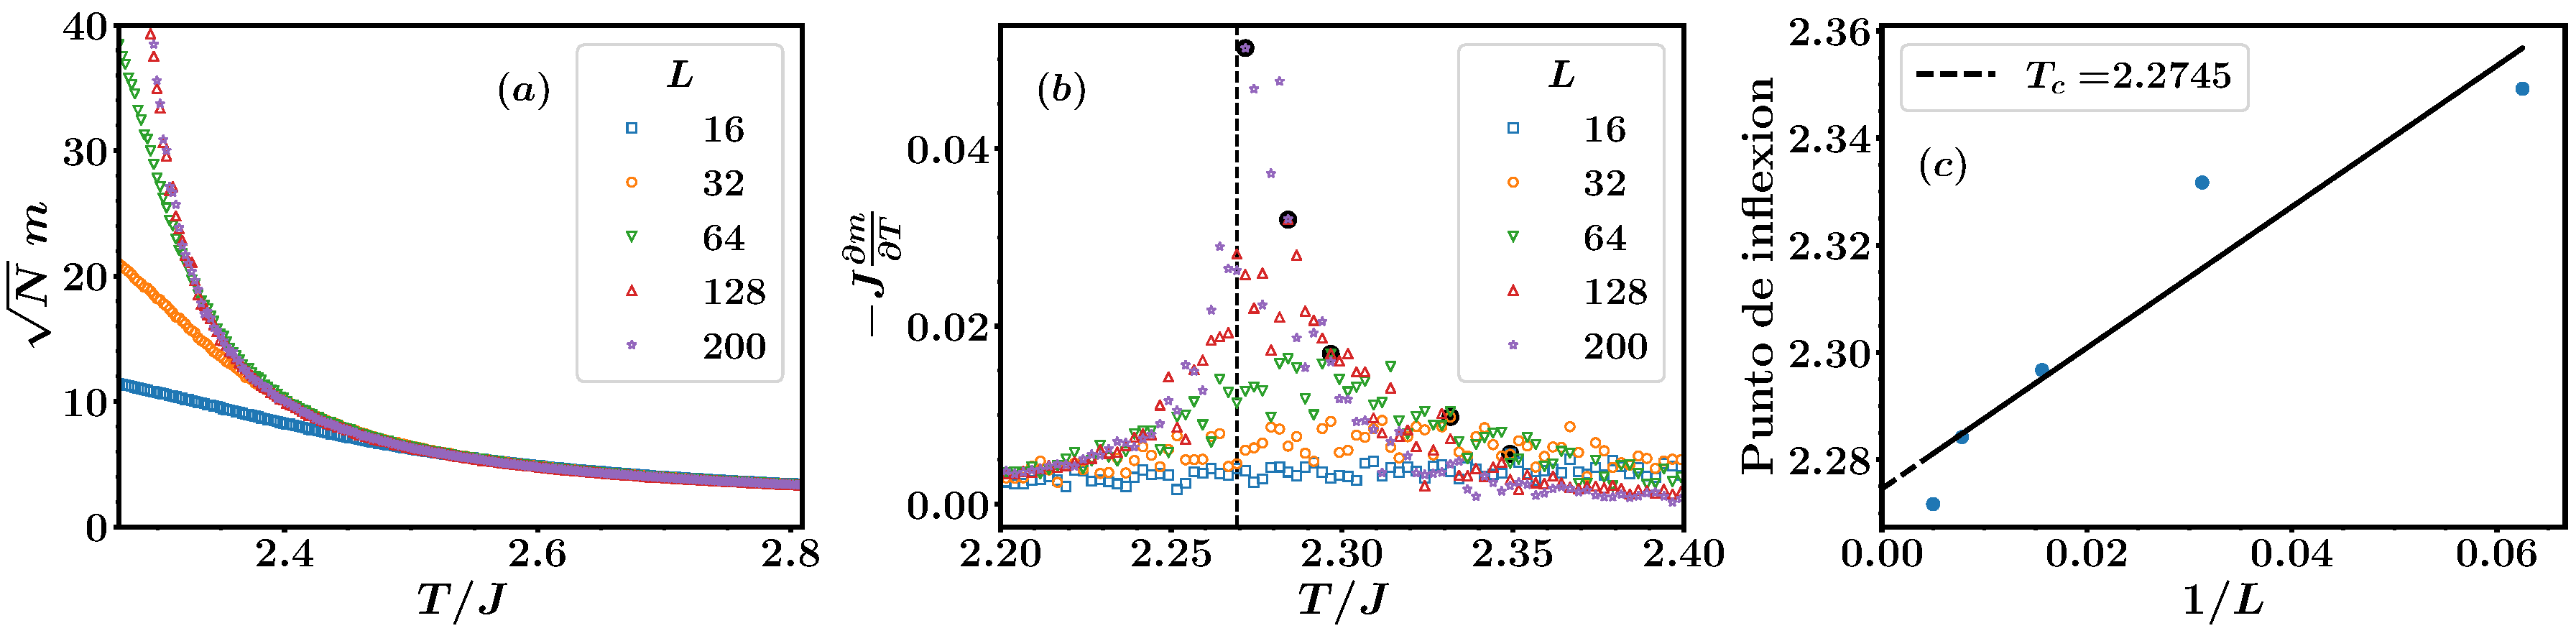
\includegraphics[scale=0.27]{Fig2.pdf}
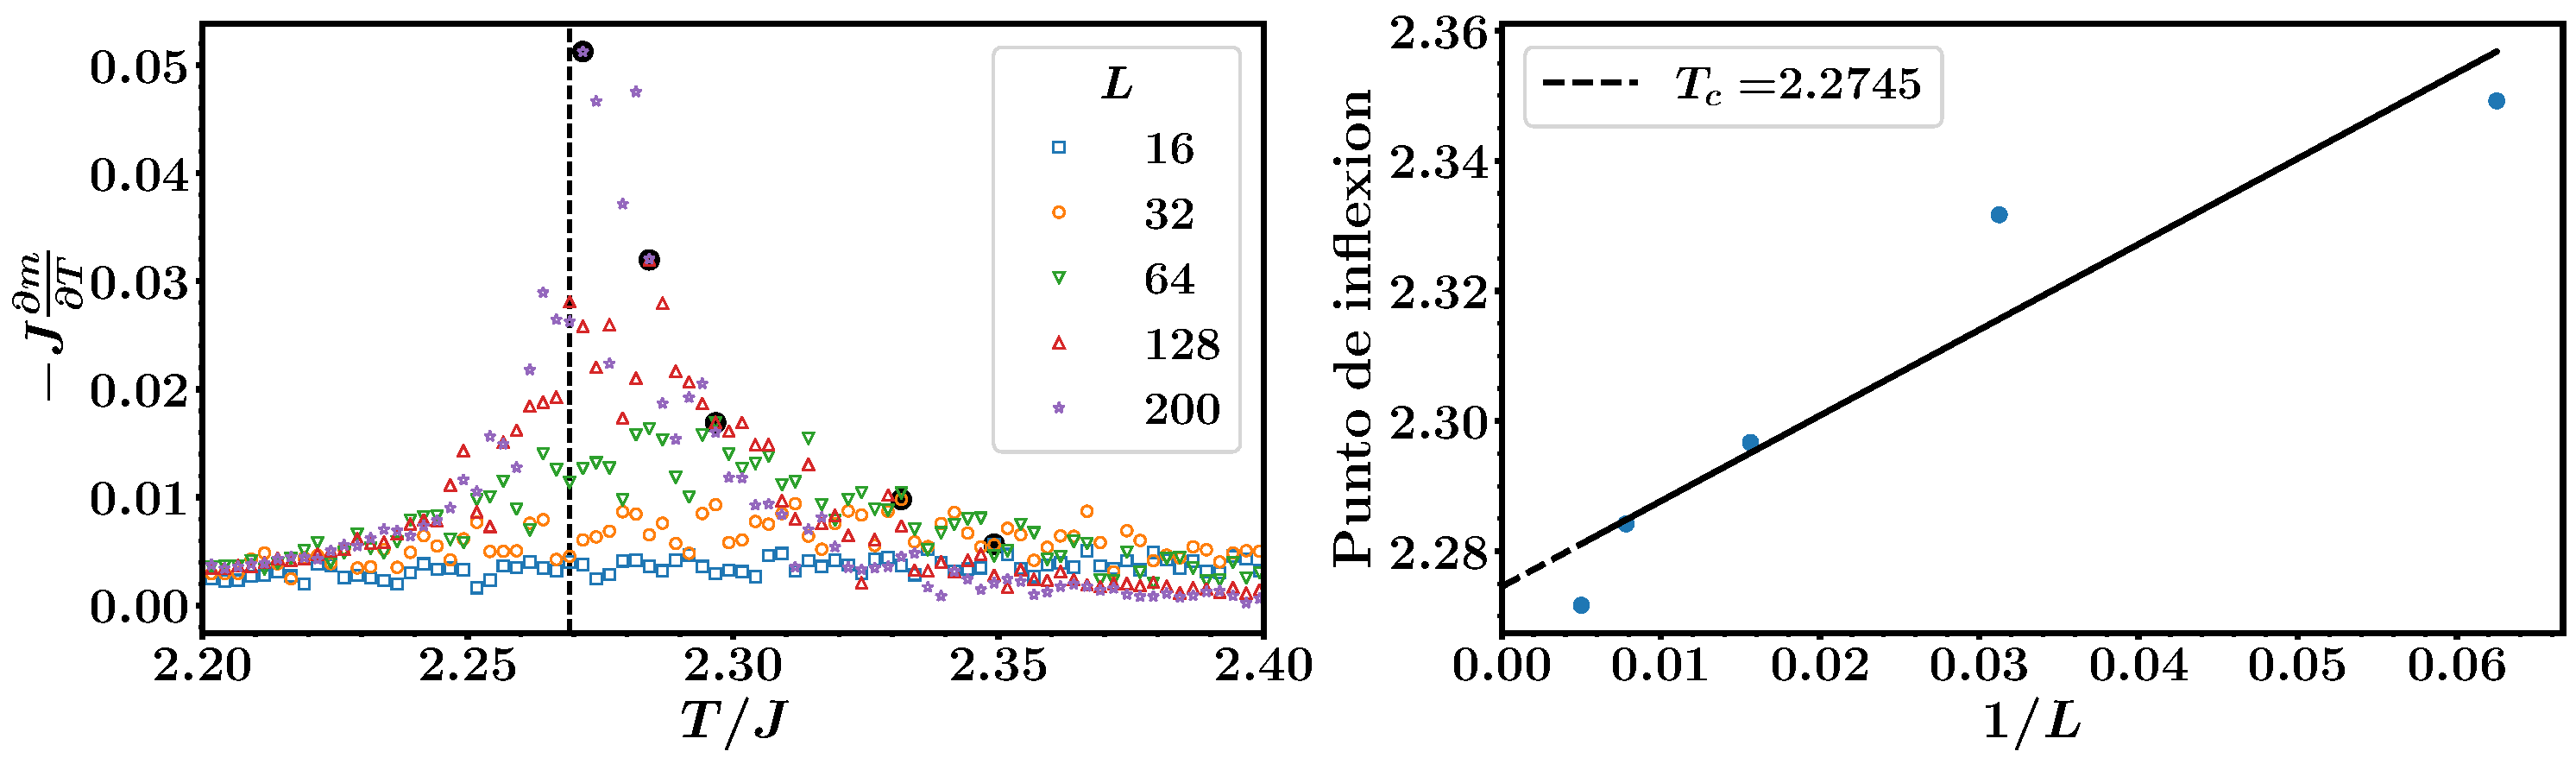
\includegraphics[scale=0.27]{Fig3.pdf}
\caption{(a) Decaimiento de la magnetización como función de la temperatura. Las curvas se superponen a partir de una determinada temperatura cuando son reescaladas por el factor $\sqrt{N}$. (b) Derivada de la magnetización con respecto a la temperatura, graficada en función de la temperatura. El punto de inflexión de las curvas de la figura (a) corresponde a los máximos de estas curvas. (c) Comportamiento de los puntos de inflexión en función de $1/L$. La recta corresponde a un ajuste lineal por mínimos cuadrados de los puntos. La ordenada al origen representa la estimación de la temperatura crítica en el límite termodinámico. El valor obtenido es $\hat{T}_c = 2.275$, ligeramente superior que el valor teórico $T_c = 2.269$.}
\end{figure}

\pagebreak

\item Usando las relaciones de escala con el tamaño finito

\begin{align}
\langle m^2 \rangle_L &\sim L^{-2\beta/\nu} F_2(Lt^{\nu}) \\
\langle m^4 \rangle_L &\sim L^{-4\beta/\nu} F_4(Lt^{\nu}), 
\end{align}

estime la temperatura crítica a través del cumulante de Binder 

\begin{equation}
U_L = \dfrac{\langle m^4 \rangle_L}{\langle m^2 \rangle_L^2}
\end{equation}

y compare con la estimación anterior.

El cumulante de Binder se define como la curtosis de la distribución de probabilidad de $M$. Es decir,

$$
U = 1 - \dfrac{\langle M \rangle^4}{3\langle M^2 \rangle^2}
$$

A temperatura cero, $U = 2/3$, mientras que a temperatura infinita, $U\rightarrow 0$.

Cerca del punto crítico, el cumulante tiene un comportamiento del tipo 

$$
U(T,L) = b(tL^{1/\nu}),
$$

donde $t = (T-T_c)/T_c$ es la temperatura reducida. Por lo tanto, las curvas de $U(T, L)$ para distintos valores de $L$ deben cruzarse en $T=T_c$.

\begin{figure}[ht]
\centering
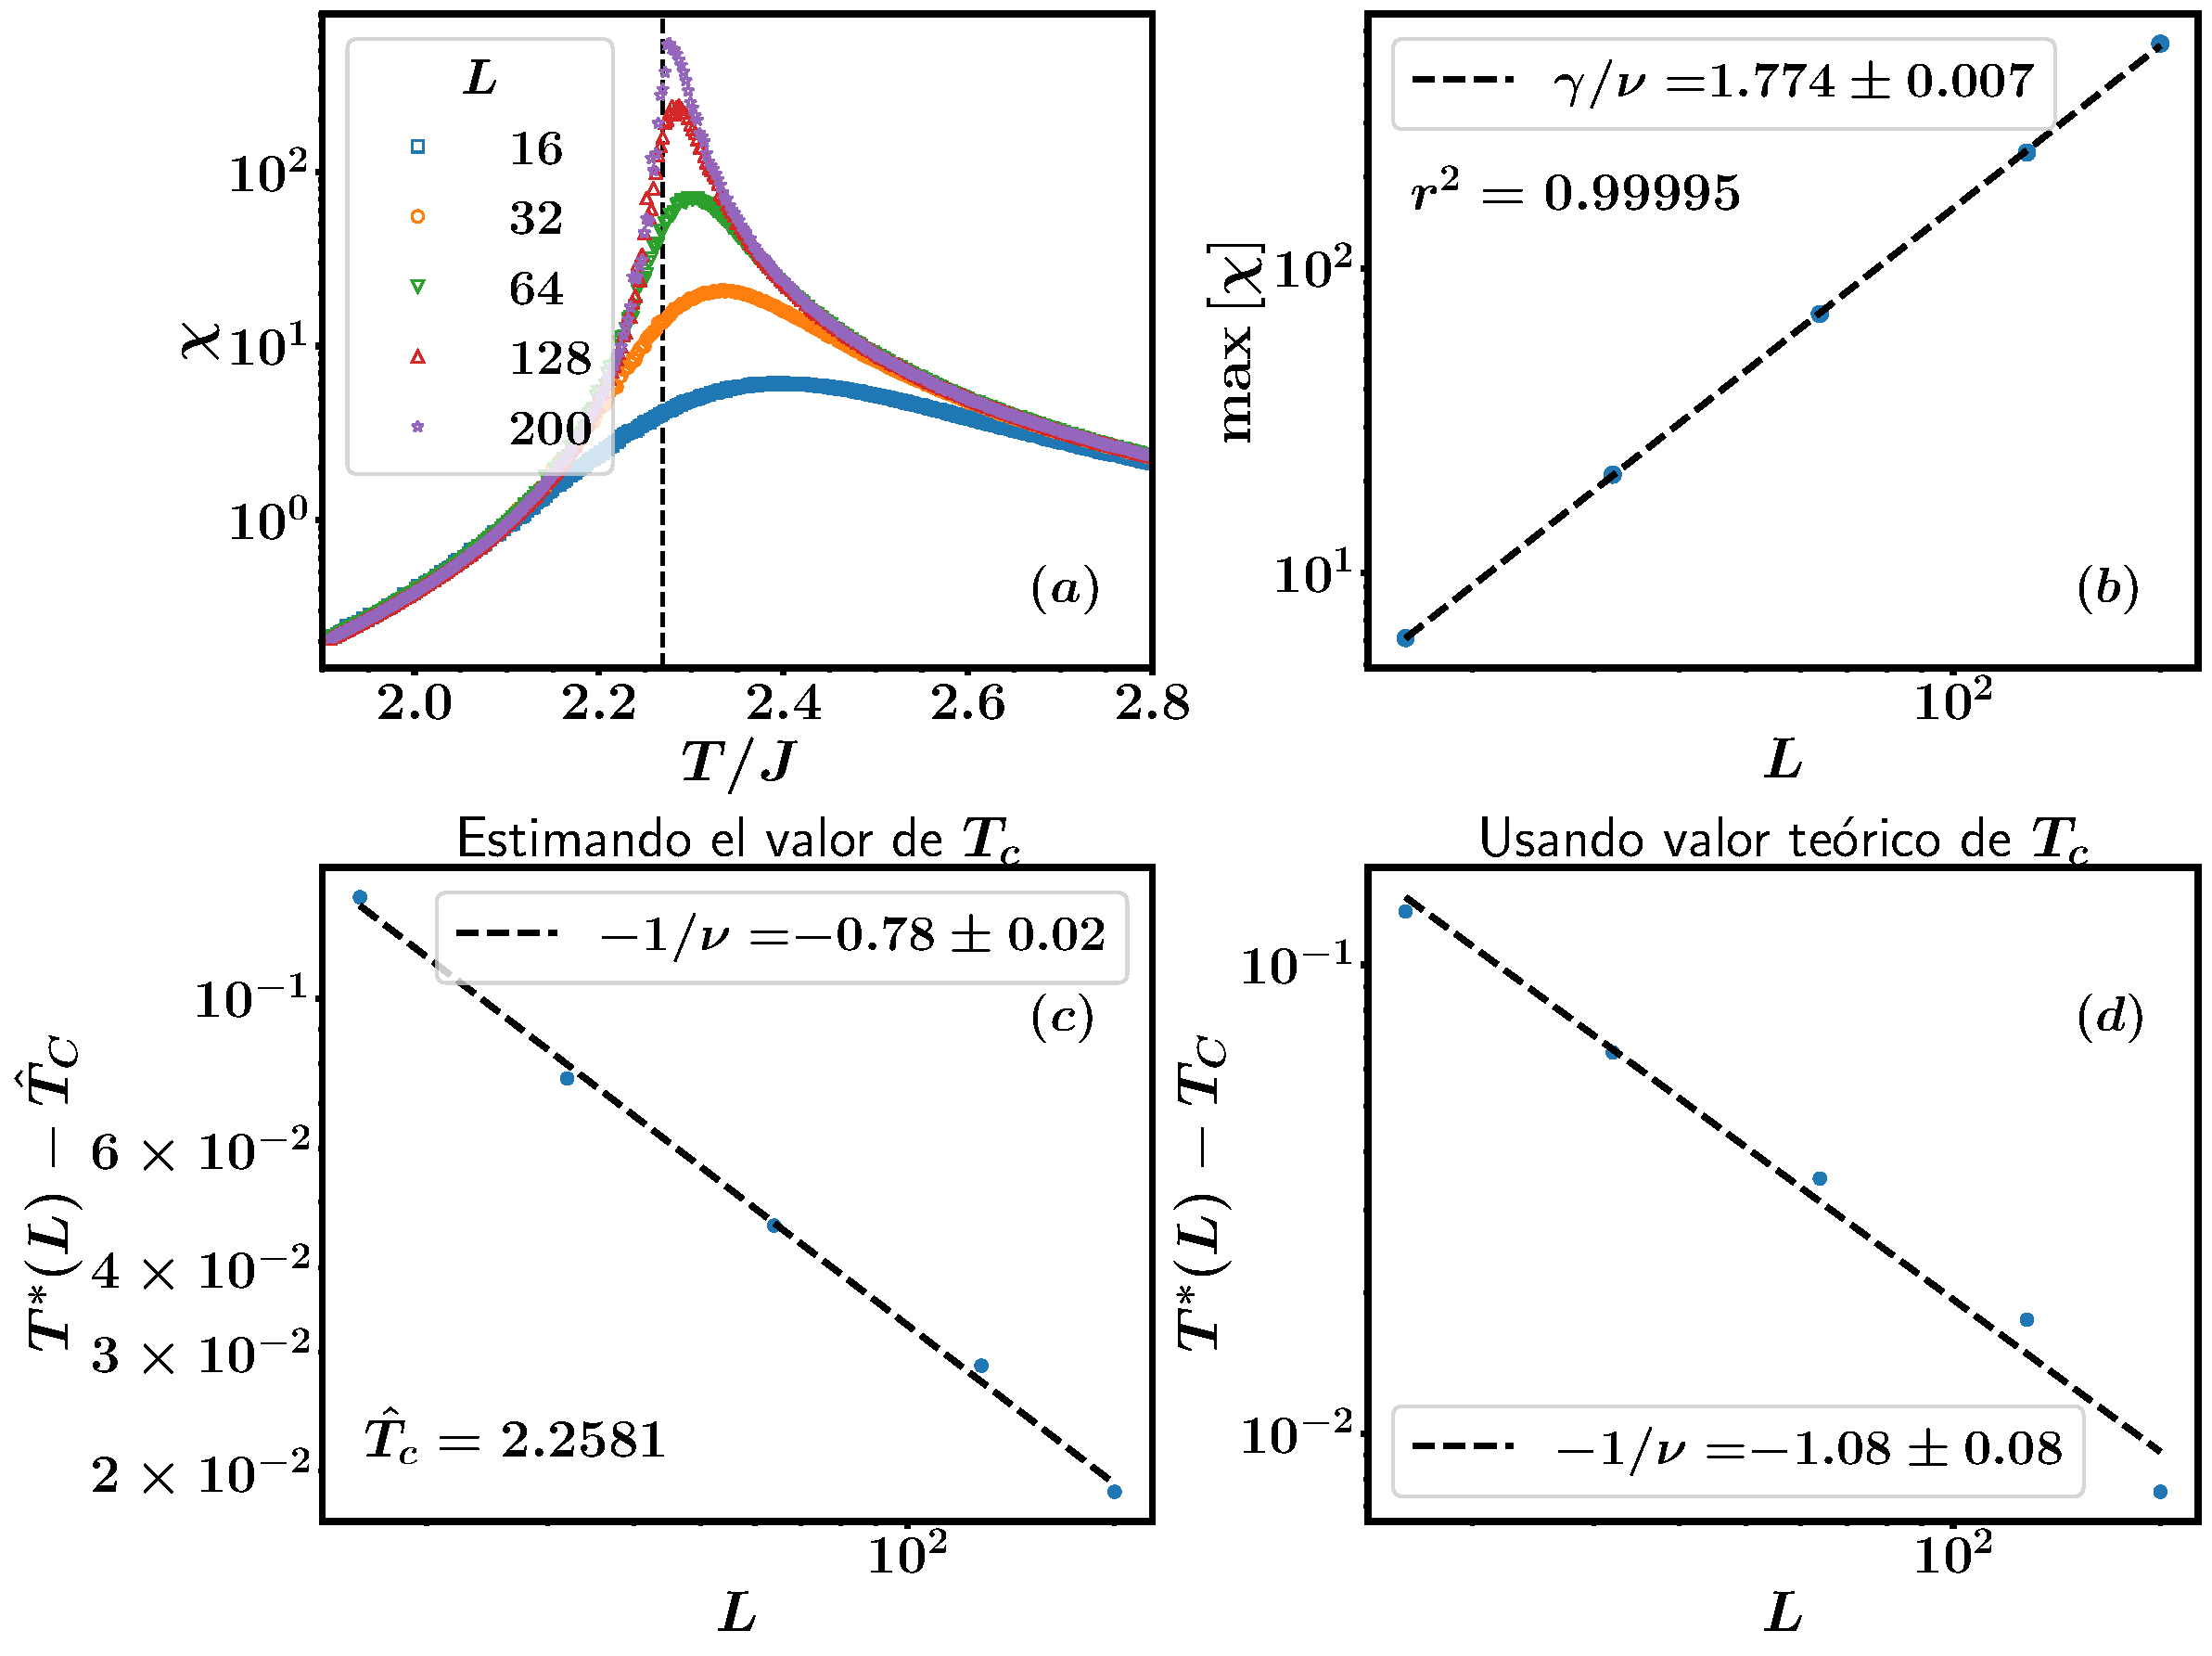
\includegraphics[scale=0.27]{Fig4.pdf}
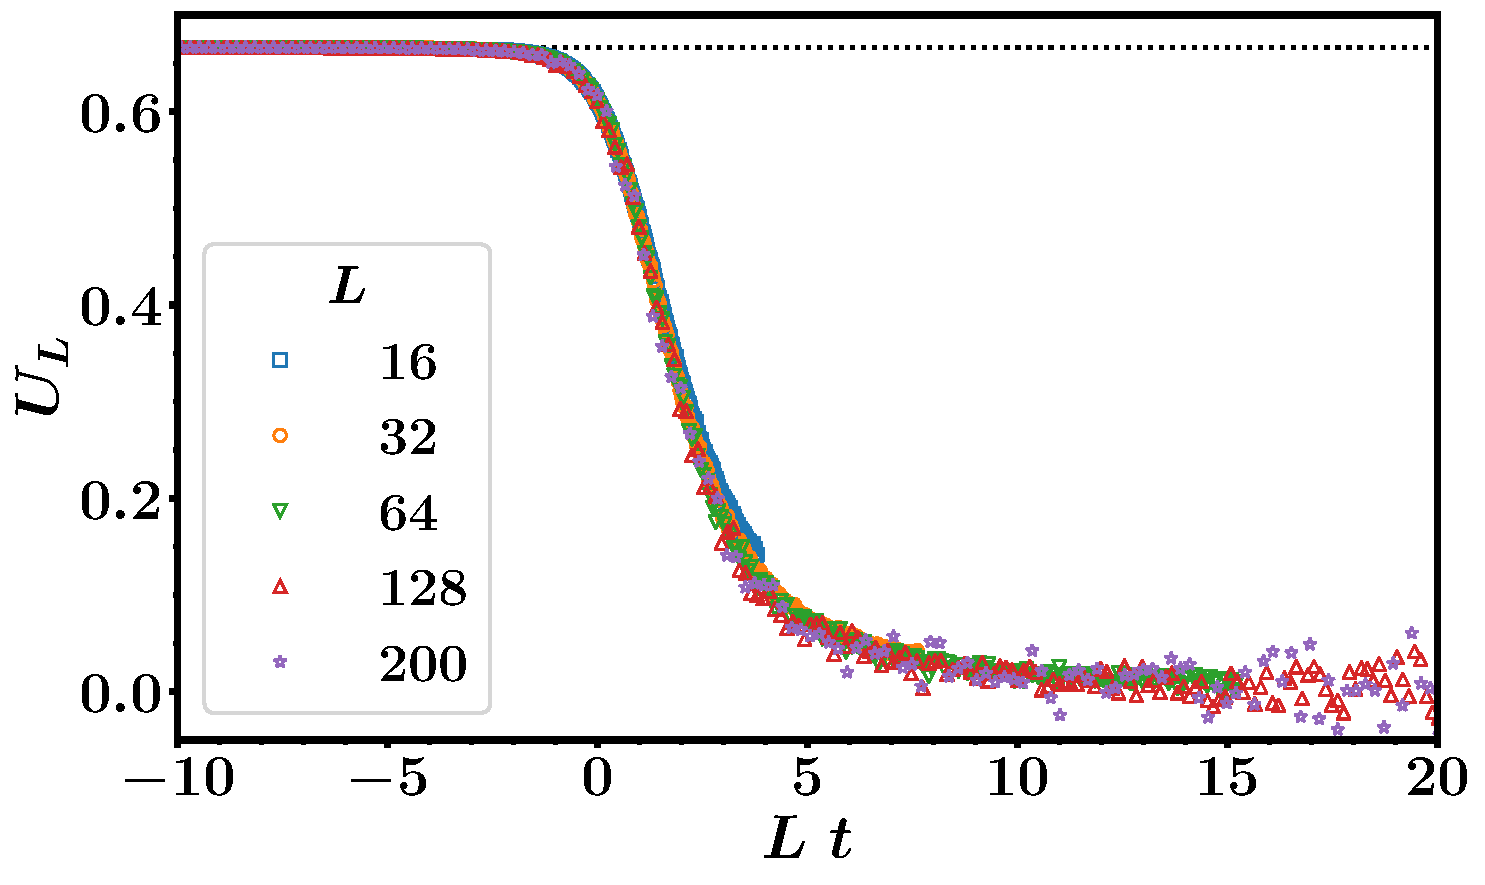
\includegraphics[scale=0.27]{Fig5.pdf}
\caption{(a) Cumulante de Binder en función de la temperatura para diferentes tamaños del sistema. El punto de intersección entre las curvas representa una estimación de la temperatura crítica. (b) Acercamiento a la intersección, cuyo valor es $\hat{T}_c = 2.269\pm 0.003$. El resultado obtenido coincide, dentro del error, con el valor teórico, por lo que el método resulta confiable. (c) Colapso de las curvas al reescalar la temperatura con el tamaño del sistema.}
\end{figure}

\pagebreak

\item Es posible que el máximo de la susceptibilidad ocurra en una temperatura pseudo-crítica $T^*(L) = T_c + A L^{1/\nu}$, donde $A$ es una constante. Además, el valor del máximo crece con el tamaño como $L^{\gamma/\nu}$. Usando estos resultados estime $\gamma / \nu$. También estime la temperatura crítica y compare el resultado con los valores obtenidos anteriormente.

\begin{figure}[ht]
\centering
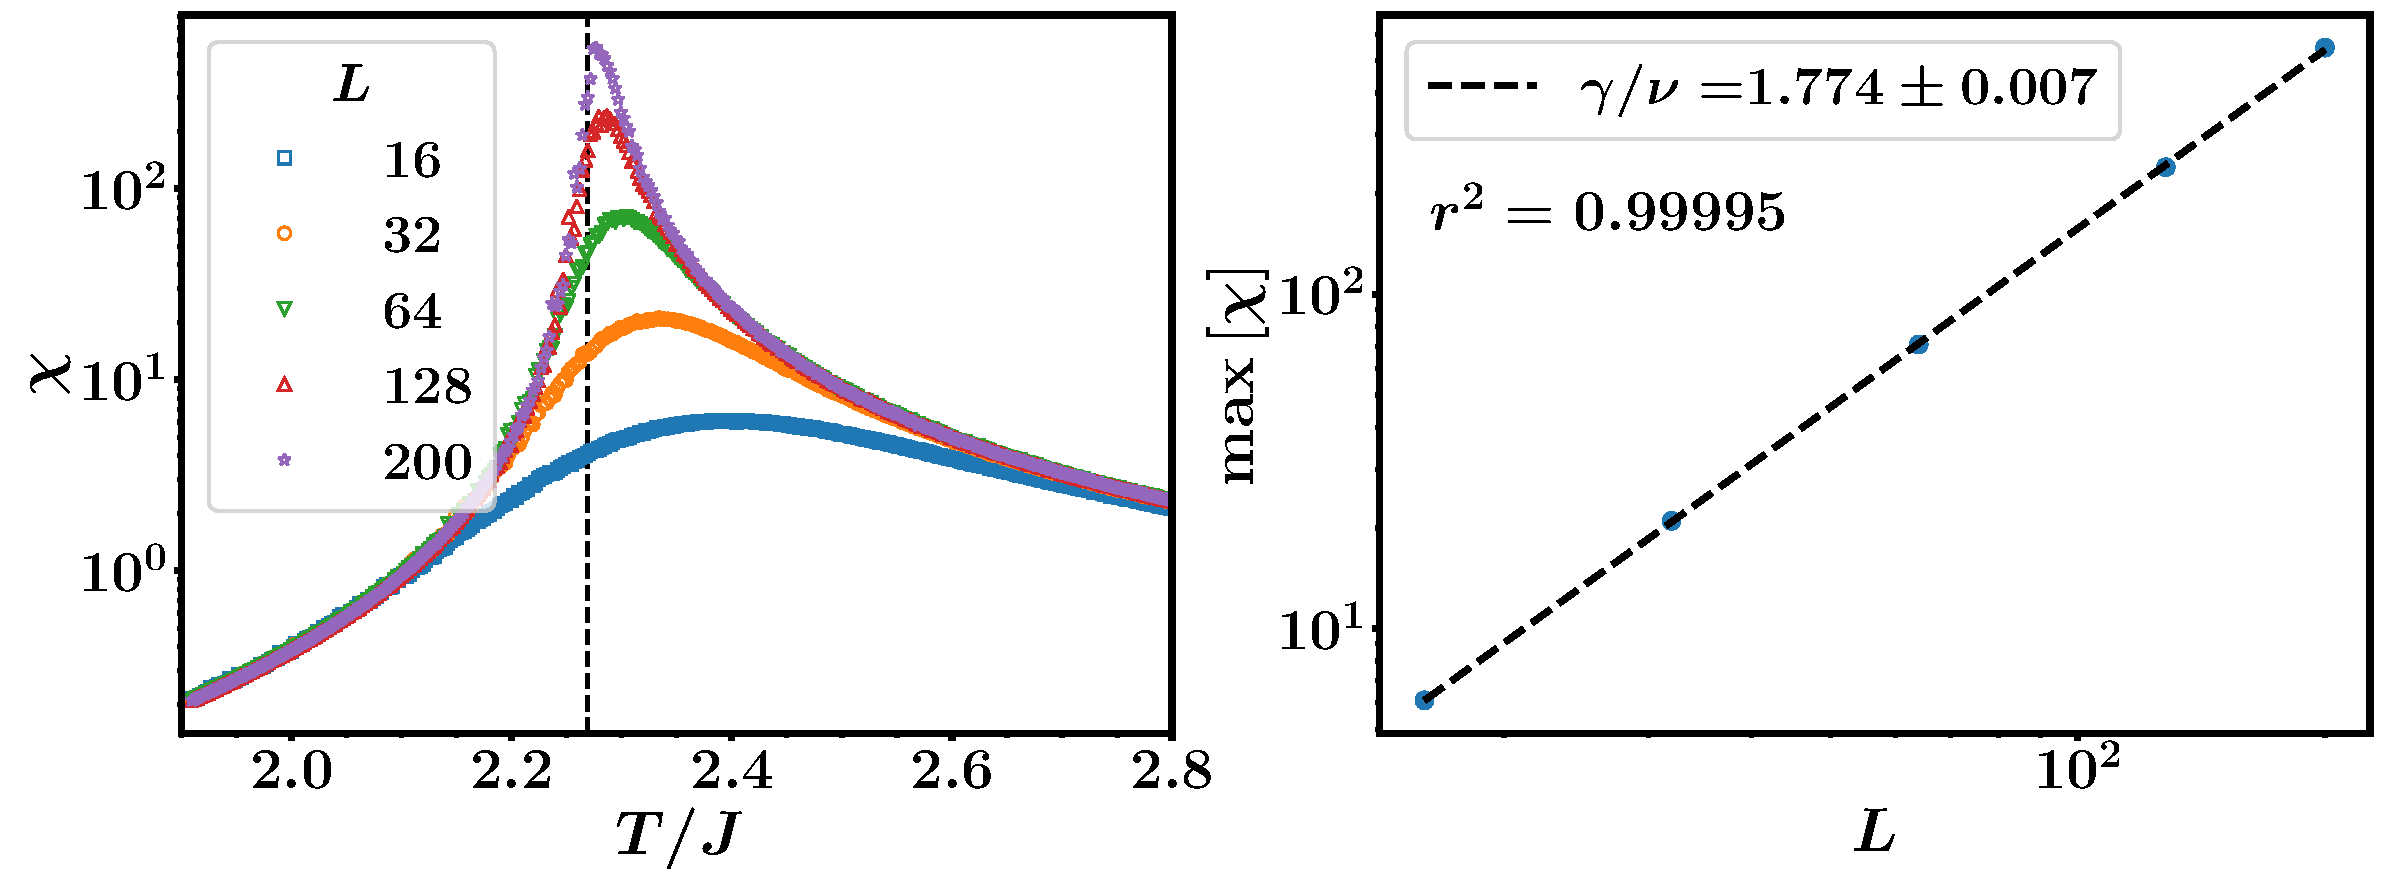
\includegraphics[scale=0.27]{Fig6.pdf}
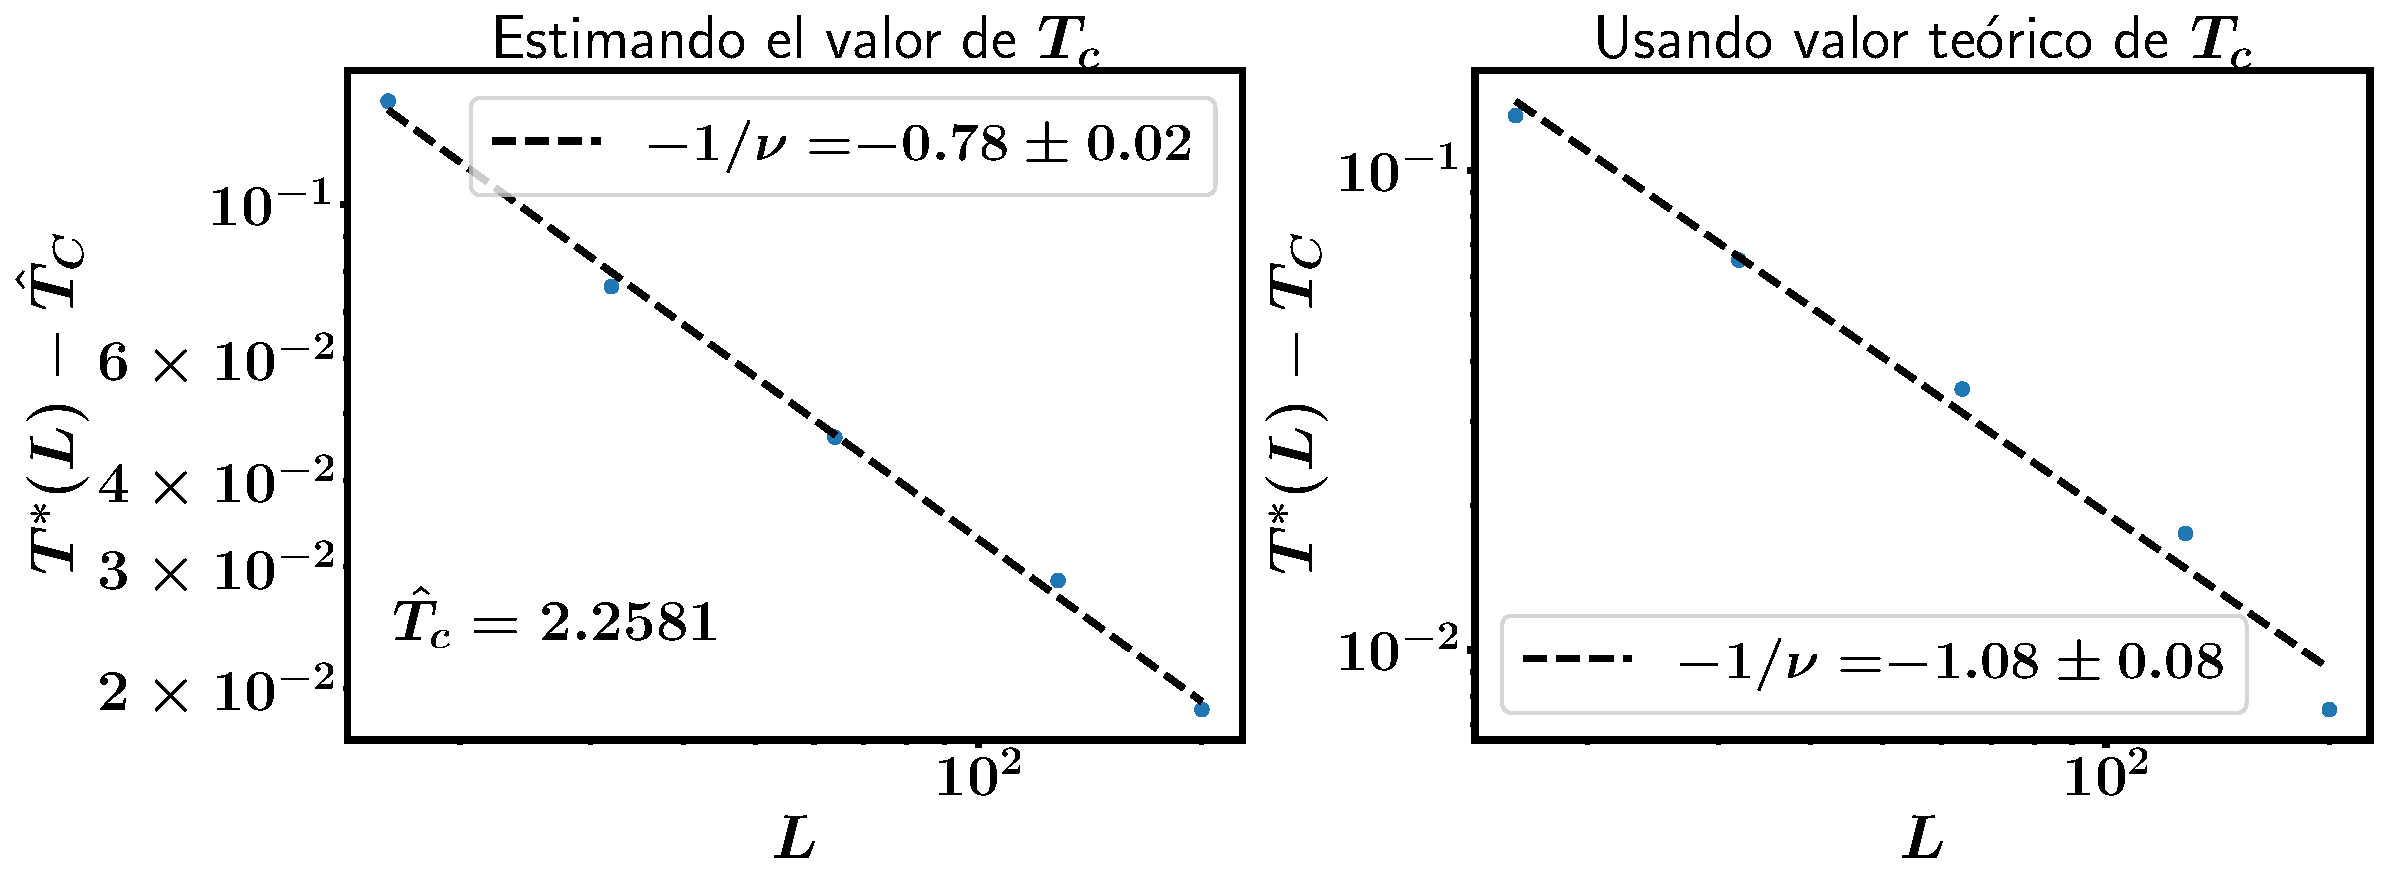
\includegraphics[scale=0.27]{Fig7.pdf}
\caption{(a) Susceptibilidad en función de la temperatura, para distintos tamaños del sistema (escala lin-log). Se puede apreciar que esta cantidad presenta un pico en un valor de $T$ que depende del tamaño, y que se sitúa por la derecha de $T_c$. A medida que el tamaño aumenta, el pico se posiciona cada vez más cerca de la temperatura crítica. (b) Valor máximo de la susceptibilidad en función del tamaño del sistema. La recta representa un ajuste por mínimos cuadrados. La pendiente de la recta permite estimar el cociente $\gamma/\nu$ como $\hat{\gamma/\nu} = 1.774\pm 0.007$. El valor obtenido es ligeramente superior que el valor teórico $\gamma /\nu = 1.75$. (c) Estimación simultánea de $T_c$ y $1/\nu$ mediante la ecuación  $T^*(L) = T_c + A L^{1/\nu}$. El procedimiento utilizado consiste en realizar un ajuste por mínimos cuadrados de $\log [T^*(L) - T]$ vs. $\log L$, barriendo valores de $T$. Definimos $\hat{T}_c$ como la temperatura que minimice el error del ajuste, en este caso $\hat{T}_c = 2.258$. Además, con la pendiente de la recta obtenemos $1/\hat{\nu} = 0.78$. Podemos ver que este método presenta un error importante en ambas estimaciones, que puede ser atribuido al hecho de ajustar los dos parámetros simultáneamente. (d) Estimación del exponente $1/\nu$ empleando la misma ecuación que en (c), pero esta vez utilizando el valor teórico de la temperatura. El valor estimado es $1/\hat{\nu} = 1.08\pm 0.08$, el cual coincide dentro del error con el valor teórico $1/\nu = 1$.}
\end{figure}

\pagebreak

\item Usando leyes de escala estime todos los exponentes críticos para el modelo de Ising en 2D y compare con los resultados exactos.

\begin{table}[ht]
\centering
\begin{tabular}{c|c|c}
 Exponente & Teoría & Estimación  \\ \hline
 $\alpha$  & 0 & $-0.16\pm 0.2$  \\
 $\beta$  & 0.125 &  $0.12\pm 0.02$ \\
 $\gamma$ & 1.75 &  $1.9\pm 0.2$ \\
 $\delta$  & 15 &  $ 16\pm 3$ \\
 $\nu$ & 1 & $1.08\pm 0.08$
\end{tabular}
\caption{Exponentes estimados y comparación con valores teóricos, teniendo en cuenta las estimaciones anteriores y las leyes de escala $\alpha + 2\beta + \gamma = 2$, $\gamma = \beta (\delta - 1)$ y $\gamma + 2\beta = d\nu$. En todos los casos, los exponentes estimados coinciden con los valores teóricos dentro de las incertezas.}
\end{table}


\pagebreak

\item Calcule la curva de magnetización en función del campo $B/J$ para distintas temperaturas por encima y por debajo de $T_c$, así como para el valor de $T_c$ estimado anteriorment. Estime a partir de estos resultados el exponente $\delta$. Grafique simultaneamente $m/|t|^{\beta}$ vs. $B/|t|^{\Delta}$, con $\Delta = \beta \delta$ y $t$ es la temperatura reducida, usando los exponentes críticos exactos y los estimados. 

\pagebreak

\item Analice cómo crece el máximo del calor específico con $L$. Asumiendo que el mismo crece con una ley de potencia $\max [C] \sim L^{\alpha/\nu}$, estime el exponente $\alpha / \nu$.


\begin{figure}[ht]
\centering
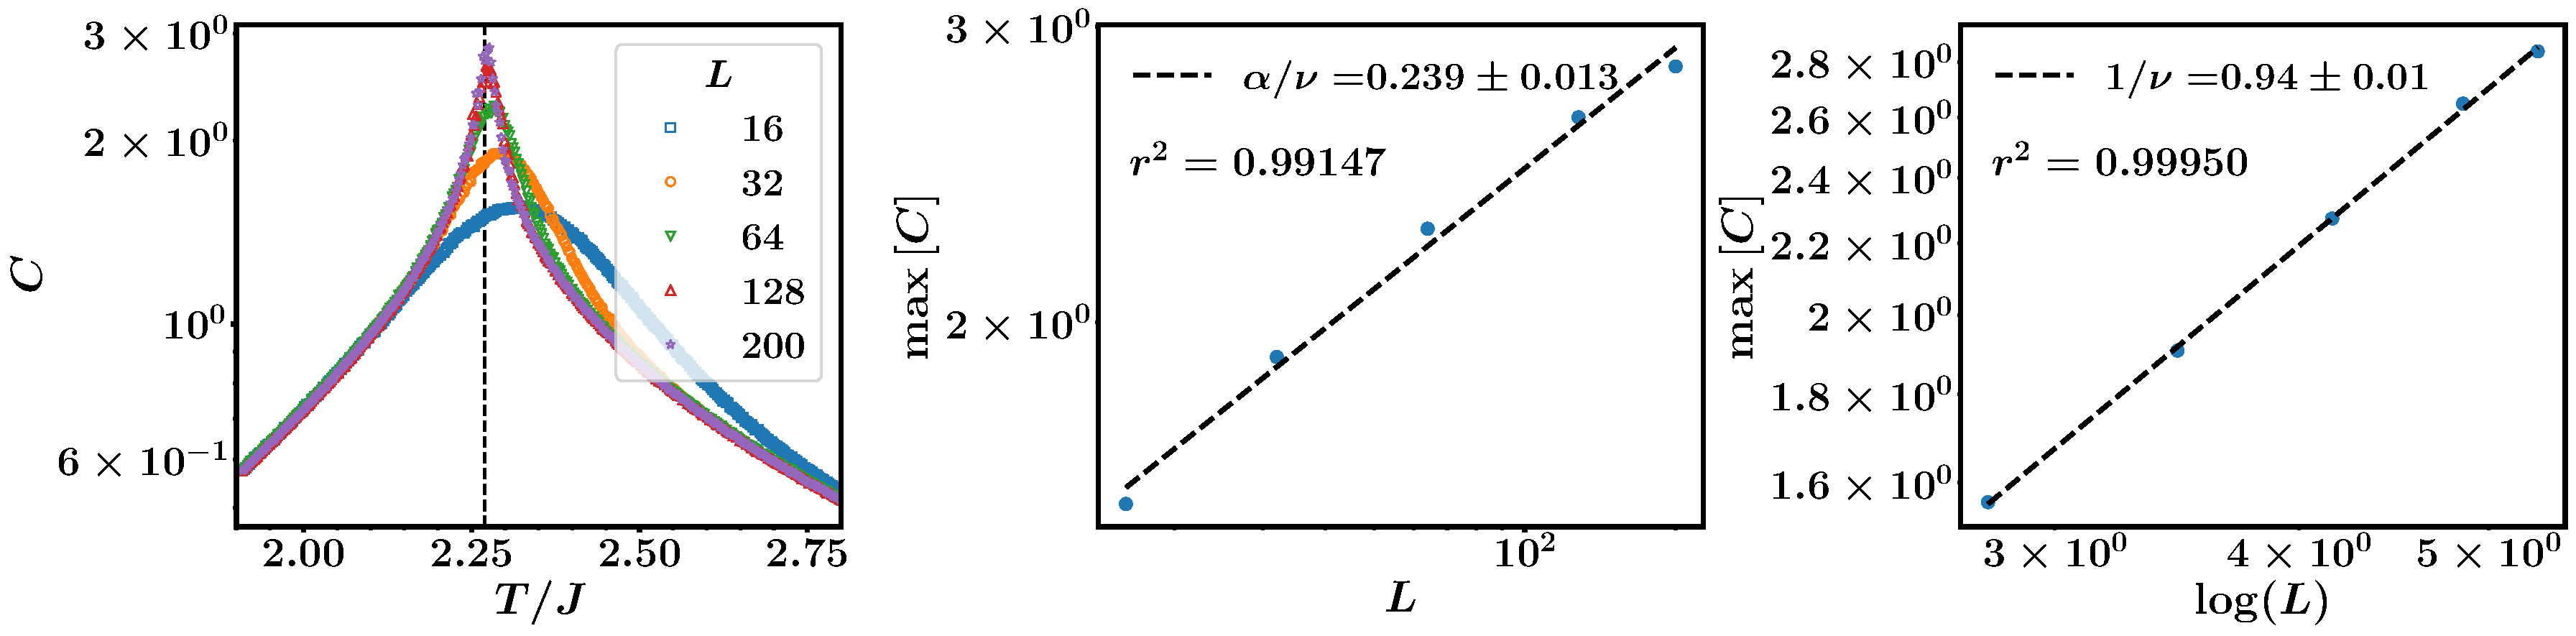
\includegraphics[scale=0.27]{Fig11.pdf}
\caption{(a) Calor específico en función de la temperatura, para diferentes tamaños del sistema. Observamos que esta cantidad presenta un pico cerca de la temperatura crítica. (b) Ajuste de los picos según la ecuación $C \sim L^{\alpha / \nu}$. Podemos ver que el ajuste no es bueno, ya que los puntos se curvan en escala log-log. Además, el cociente entre exponentes hayado no concuerda con el valor teórico. (c) Ajuste de los picos suponiendo un escaleo logarítmico de la forma $C \sim \dfrac{1}{\nu}$ (es decir, tomando $\alpha = 0$). En este caso, el ajuste es mejor, y el estimador para el exponente $1/\nu$ hayado se aproxima más al valor teórico.}
\end{figure}

\end{enumerate}



\end{document}
